%%%%%%%%%%%%%%%%%%%%%%%%%%%
%                         %
%       2016.11.16.       %
%      Szakdolgozat       %
%    Tamás     LATEX      %
%%%%%%%%%%%%%%%%%%%%%%%%%%%
\documentclass[oneside,titlepage,12pt,a4paper]{report}
%\documentclass[12pt]{report}
\usepackage[centertags]{amsmath}
\usepackage{amsfonts}
\usepackage{amsthm}
\usepackage{newlfont}
%\usepackage[ansinew]{inputenc}
\usepackage[magyar]{babel}	
\usepackage[utf8]{inputenc}		
\usepackage{t1enc}				
\usepackage{graphicx}
\usepackage{color}
%\usepackage[colorlinks]{hyperref}
%\usepackage[active,new,noold,marker]{xrcs}
\usepackage{euler}
\usepackage{amssymb,latexsym}
\usepackage{amsmath}
\usepackage{graphics}
\usepackage{algorithm} 
%\usepackage{algpseudocode} %ezzel összeakadhat \usepackage{algorithmic} 
\usepackage{rotating}
\usepackage{bigstrut}
\usepackage{subfigure}
\usepackage{appendix}
\usepackage{setspace}


\newtheorem{theorem}{Theorem}
\newtheorem{corollary}{Corollary}
\newtheorem{lemma}{Lemma}
\newtheorem{proposition}{Proposition}
\newtheorem{definition}{Definition}
\newtheorem{notation}{Notation}

\textwidth=6.truein \textheight=9.truein \hoffset=-.5truein
\voffset=-.8truein

\frenchspacing				
\setlength{\parskip}{\smallskipamount}	
\renewcommand{\appendixtocname}{Függelék}
\renewcommand{\appendixpagename}{Függelék}
\DeclareMathOperator{\grad}{grad}
\DeclareMathOperator{\sgn}{sign}
\DeclareMathOperator{\PRD}{PRD}
\DeclareMathOperator{\CR}{CR}
\newcommand{\conj}[1]{\overline{#1}}

\begin{document}
\begin{titlepage}
	\parbox[t]{5.5cm}{\vspace{1cm}}
\begin{center}
	\large
	\textsc{Eötvös Loránd Tudományegyetem \linebreak Informatikai Kar} \\[2cm]
\end{center}

\begin{center}
	% Title
	\LARGE EKG jelek feldolgozása Hermite-függvények segítségével\\[0.55cm]
	\large BSc Szakdolgozat \\[1.9cm]
\end{center}

\begin{center}
	\parbox[t]{25mm}{Készítette:}
	\parbox[t]{5.5cm}
		{Dózsa Tamás\\
		ELTE IK\\
		Programtervező informatikus \\
		BSc
		}
	\\[0.9cm]
	
  \parbox[t]{25mm}{Témavezető:}
	\parbox[t]{5.5cm}{
		Dr. Kovács Péter\\
		Adjunktus\\
		ELTE IK\\
		Numerikus Analízis Tanszék
		}
	\\[4cm]
\end{center}

\begin{center}
	
\includegraphics[scale=0.7]{./Abrak/Egyeb/elte_logo.jpg}\\[1cm]
	Budapest, 2016.11.16.
\end{center}
\end{titlepage}

\tableofcontents

%%%%%%%%%%%%%%%%%%%%%
% BEVEZETES
%%%%%%%%%%%%%%%%%%%%%

\chapter{Bevezetés}
\label{intro}

\paragraph{}
Az információ ábrázolásának módja az informatika tudomány fontos kérdése. Természetesen annak eldöntése, hogy egy adott adat halmaz milyen módon kerül ábrázolásra erősen függ annak jellegétől. Az adatábrázolás felel az adatok hatékony felhasználhatóságáért (például egy internetes video hívásnál az adatokat gyorsan kell egymás után továbbítani), ugyanakkor biztosítania kell, hogy az adatokból kinyerhető információ nem veszik el (ha túl rossz mindőségű képeket továbbítunk, a fogadó fél nem tudja értelmezni azokat). 
\paragraph{}	A szakdolgozat célja egy speciális adatábrázolás, nevezetesen EKG jelek egy ábrázolásának bemutatása. Mivel jellemzően ezeket az adatokat, későbbiekben \textit{jelek}-et, általában nagyobb memória felhasználásával szokás ábrázolni, ezért a dolgozat az eljárásra EKG jelek \textit{tömörítéseként} hivatkozik. EKG jelek esetén az ábrázolás minősége sok szemponttól függ. Mivel ezek a jelek fontos információkat hordoznak a szív állapotáról, különösen fontos, hogy a tömörítés során ne vesszen el fontos információ. Egy ilyen jel rögzítésekor azonban sok olyan adat is tárolásra kerül (például a végtagok mérés közbeni mozgatása miatt), amelyek nem hordoznak fontos információt. Az ilyen adatokra a dolgozat \textit{zaj}-ként hivatkozik. Egy jó EKG ábrázolás sikeresen szűri a mérés során keletkezett zajt, miközben az orvosi szempontból fontosnak nevezhető információt megtartja. Mivel a dolgozatban egy tömörítési eljárás kerül bemutatásra, fontos szempont az EKG jelek memória takarékos ábrázolása. Gyakorlati szempontból minél kevesebb memórián történik meg a jelek ábrázolása, annál könnyebb azokat tárolni (hosszú mérések esetén fontos lehet), illetve egyszerűbb és biztonságosabb a jelek hálózaton törtenő továbbítása. EKG jeleknek egy igazán jónak nevezhető ábrázolása pedig az eddig említettek mellett az orvosok munkáját közvetlenül segítő információt is kódol magában. Ilyen lehet például egy olyan ábrázolás amely hatékony bemenetéül szolgál valamilyen osztályozó algoritmusnak, lehetővé téve az abnormális jelek automatikus felismerését. 
	\paragraph{} A dolgozat három fő fejezetre tagolható. A Bevezetés című fejezetben található a dolgozatban bemutatott eljárás specifikációja, a jel reprezentáció matematikai modelljének ismertetése, valamint a bemutatott módszer egyéb jellemzőit ismertető alfejezetek. Ezek közé tartozik például a jel közelítésének optimalizációjához szükséges Nelder-Mead algoritmus elméleti bemutatása, illetve az EKG jel szegmentációját elősegítő Matching-Pursuit algoritmust részletező alfejezet. 
\paragraph{}	A dolgozat második fejezete az eljárás mellékelt implementációjának a fejlesztői dokumentációja. Ebben a fejezetben találhatóak a tömörítő eljárást implementáló c++ osztályok jellemzői, illetve az elérést segítő webes felület implementációjának részletes ismertetése. A fejlesztői dokumentáció fejezet tartalmazza továbbá a program logikai jellemzését elősegítő UML és egyéb osztálydiagrammokat. A fejezet igyekszik pragmatikusan és érthetően jellemezni a program felépítését, illetve kellően megindokolni az egyes implementációk mellett szóló döntéseket. 
\paragraph{}	A Felhasználói dokumentáció fejezetbe, a program használatával kapcsolatos információk kerültek. Ebben a fejezetben található a felhasználói felület funkcióinak pontos ismertetése, valamint hasznos példák annak használatára. Bemutatásra kerülnek továbbá a program használatához szükséges előkészületi lépések, és az ismert rendszerkövetelmények. 
\paragraph{}	A dolgozat utolsó része a függelék, melyben a Bevezetés fejezetben található matematikai állítások bizonyításai, egyéb kapcsolódó matematikai fogalmak leírásai, illetve felhasznált algoritmusok pszeudo-kódja található. 
		
\section{A feladat specifikációja}

A dolgozat célja egy olyan tömörítési eljárás bemutatása, amely lehetővé teszi az EKG jelek hatékony (memória takarékos) ábrázolását, a mérések zaj szűrését, illetve az EKG hullámszegmenseinek szeparációját. Az utóbbi jellemző orvosi szempontból lehet hasznos, ugyanis sok kóros elváltozás kimutatásához szükséges az egyes hullámszegmensek széleinek ismerete. A dolgozatban bemutatott módszer hatékonysága, az irodalomban fellelhető más tömörítési eljárások \cite{} hatékonyságának összehasonlításával igazolandó. A dolgozatban bemutatott tömörítési eljárás implementációjának feladata, hogy az MIT-BIH adatbázisban található EKG jelek tömörítésére alkalmas legyen, ehhez pedig egy könnyen használható webes felületet biztosítson. A bemutatott tömörítési eljárás implementációjának két féle bemente megengedett: tömörítés esetén az MIT-BIH adatbázisban megtalálható EKG jelek, illetve a tömörítés következtében létrejött számsorozat, melyet a tömörített jel helyreállításához használ.  

\section{A modell ismertetése}
A modern orvostudományban nagy jelentőséggel bírnak 
a valamely élő szervezet által kibocsátott úgynevezett $biológiai jelek$. Ezek közé sorolható az $Elektro$ $Kardio$ $Gram$, vagy $EKG$,
amely a szív állapotáról képes információt adni. B\'ar ennek a dolgozatnak nem célja az $EKG$ jelek pontos elemzése, fontos néh\'any sorban ismertetni egy \'atlagos $EKG$ jel meghat\'arozó hull\'amait. Egyetlen szí vütés  $EKG$ reprezent\'aciója h\'arom fő részre bontható: a szí vütés elején megjelenő $P$ hull\'amra, az ezt követő $QRS$ komplexumra, és az ütés végén tal\'alható $T$ hull\'amra. Ezek rendre a pitvari összehűzódást, a kamrák depolarizációját és elektromos újratöltődését reprezentálják. Diagnosztikai szempontból a $QRS$ komplexus a legfontosabb, ezért ezt nagy pontossággal kell tárolni. Általánosságban elmondható, hogy ezeknek a hullámoknak kezdő és végpontjai, valamint maximum és minimum értékei vesznek részt az orvosi diagnosztikában. Az említett paraméterek az \ref{fig:ekg} ábrán láthatóak.

\begin{figure}[htb!]
\begin{center}
   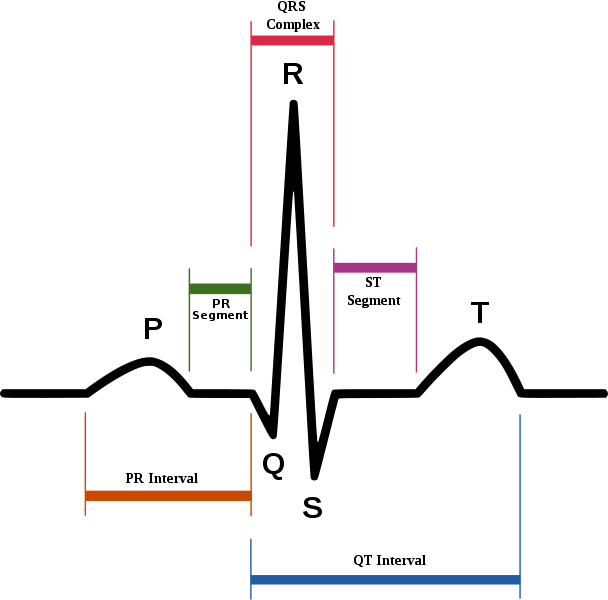
\includegraphics[scale=0.37]{./Abrak/Egyeb/ecg_wiki.png}
   \caption{Az EKG jel egy szívütése, illetve annak főbb diagnosztikai jellemzői.}
		\label{fig:ekg}
\end{center}
\end{figure}
 
Az irodalomban ismert tömörítő algoritmusokat \cite{unifiedReview} alapján három kategóriába sorolhatjuk: 1) egyszerű paraméteres becslések (pl.: interpoláció, különbségi kódolás, stb.), 2) direkt módszerek (pl.: csúcsok, meredekségek, stb. tárolása), 3) transzformációs eljárások. Az utóbbi osztály tartalmazza azokat az algoritmusokat, melyek a jelet egy előre adott függvényrendszer szerinti sorfejtéssel approximálják. Így az eredeti adatsorozat helyett csak az együtthatókat és a rendszer paramétereit kell tárolnunk. Ezen kategóriába sorolandó a dolgozatban bemutatott algoritmus is. Nevezetesen, az eredeti adatsorozatot speciális, Hermite-polinomok segítségével előállitott függvényrendszerrel fogjuk közelíti. A módszer alapját képező eljárás \cite{hexp3}, jól ismert az irodalomban, mely nem csak a jelek tömörítéséhez, de azok modellezéséhez \cite{hexp2}, illetve osztályozásához \cite{hexp1, hexp4} is alkalmazható. A dolgozatban az EKG jelekkel való hasonlóságuk miatt Hermite-függvényeket használunk az adatok reprezentálásához. Ezeket egy argumentum transzformáción keresztül szabad paraméterekkel egészítjük ki. Ennek köszönhetően az eredeti jelet egy adaptív bázisban írhatjuk fel. Az említett paraméterek megválasztásához a Nelder-Mead optimalizációs eljárást alkalmaztuk. Mivel az EKG jelek diszkrét adatsorozatok, ezért a módszert \cite{hexp5} alapján implementáltuk diszkrét ortogonális Hermite-polinomokra is. A dolgozatban különböző tesztekkel demonstráljuk az algoritmus hatékonyságát. Ehhez, több órányi, zajjal terhelt, valódi EKG felvételt használtunk. Ezen keresztül a bemutatott módszert összehasonlítottuk több másik, az irodalomban jól ismert tömörítő algoritmussal is \cite{jpeg2000ECG}. 

A tömörítő eljárást egy c++ nyelven megírt, objektum elvű alkalmazás implementálja, melyet egy webes felületen keresztül érhetünk el. A felület lehetőséget biztosít a dolgozatban jelölt tesztek újrafuttatására, valamint a teszteléskor felhasznált adatbázis további jeleinek a tömörítésére. Szintén a webes felületen keresztül nyílik alkamunk a már tömörített EKG jelek helyreállítására. 

Az alkalmazás megetrvezésekor külön hangsúlyt kapott a kód újra felhasználhatósága. Ennek érdekében a felhasznált algoritmusok, illetve matematikai modellek a lehető legáltalánosabb formában lettek implementálva. Fontos szempontot jelentett továbbá a c++11-es nyelvszabvány által nyújtotta lehetőségek minél hatékonyabb kihasználása. Jó példa erre a lambda függvények alkalmazása az optimalizációs algoritmusok implementációja során. A hatékony működés mellett azonban a program igyekszik megfelelni a modern felhasználók igényeinek. Ennek érdekében a felhaszálói felület weboldalként lett implementálva. A rendszerfüggetlen, és installáció mentes elérés lehetővé teszi a gyors és egyszerű használatot, valamint az eredmények megosztását.  

\section{Matematikai háttér}
\subsection{Jelek approximációja}

EKG jelek feldolgozásakor sok esetben szembesülünk gyakorlati kihívásokkal. Két sűrűn előforduló példa a hosszú mérések tárolása, valamint a zajjal terhelt mérések ábrázolása. Ezekre a nehézségekre egyszerre ad kielégítő megoldást, ha a jeleket  valamely $\mathcal H$ Hilbert-tér sima függvényeiből álló $(\Phi_n, n\in\Bbb N)$ ortogonális bázisában reprezentáljuk és a jelet véges sok $\Phi_0,\Phi_1,\cdots,\Phi_n$ bázisbeli elem lineáris kombinációjával közelítjük. Az $f\in\mathcal H$ jel
legjobb közelítését a tér $\|\cdot\|$ normájában az
$$
S_nf:=\sum_{k=0}^n\langle f,\Phi_k\rangle \Phi_k
$$
leképezés nyújtja, ahol $\langle\cdot,\cdot\rangle$ az $\mathcal  H$ tér
skaláris szorzatát jelöli. A jel és a közelítés eltérésének négyzete  a
$$
\|f-S_nf\|^2=\|f\|^2-\sum_{k=0}^n|\langle f,\Phi_k\rangle|^2
$$
képplettel adható meg. Adott hibán belüli közelítést véve a jel helyett  elég az
$S_nf$ approximációt reprezentáló  $\langle f,\Phi_k\rangle\ (k=0,1,\cdots, n)$ Fourier-együtthatókat tárolni.  Zajos jel esetén az ilyen típusú approximáció szűrőként is szolgál.  A közelítés megvalósításához a klasszikus ortogonális rendszerek közül  EKG görbék közelítésére  az Hermite-féle függvények bizonyultak használhatónak. Ezt támasztják alá a [...] dolgozatok. Az  Hermite függvények alkalmazása azzal is indikolható, hogy grafikonjuk hasonlít az EKG görbékre. Ezt a tulajdonságot a \ref{fig:phi0-3} ábra szemlélteti.

%\begin{figure}
%  \centering
%\subfigure[$\Phi_{0}(x)$]{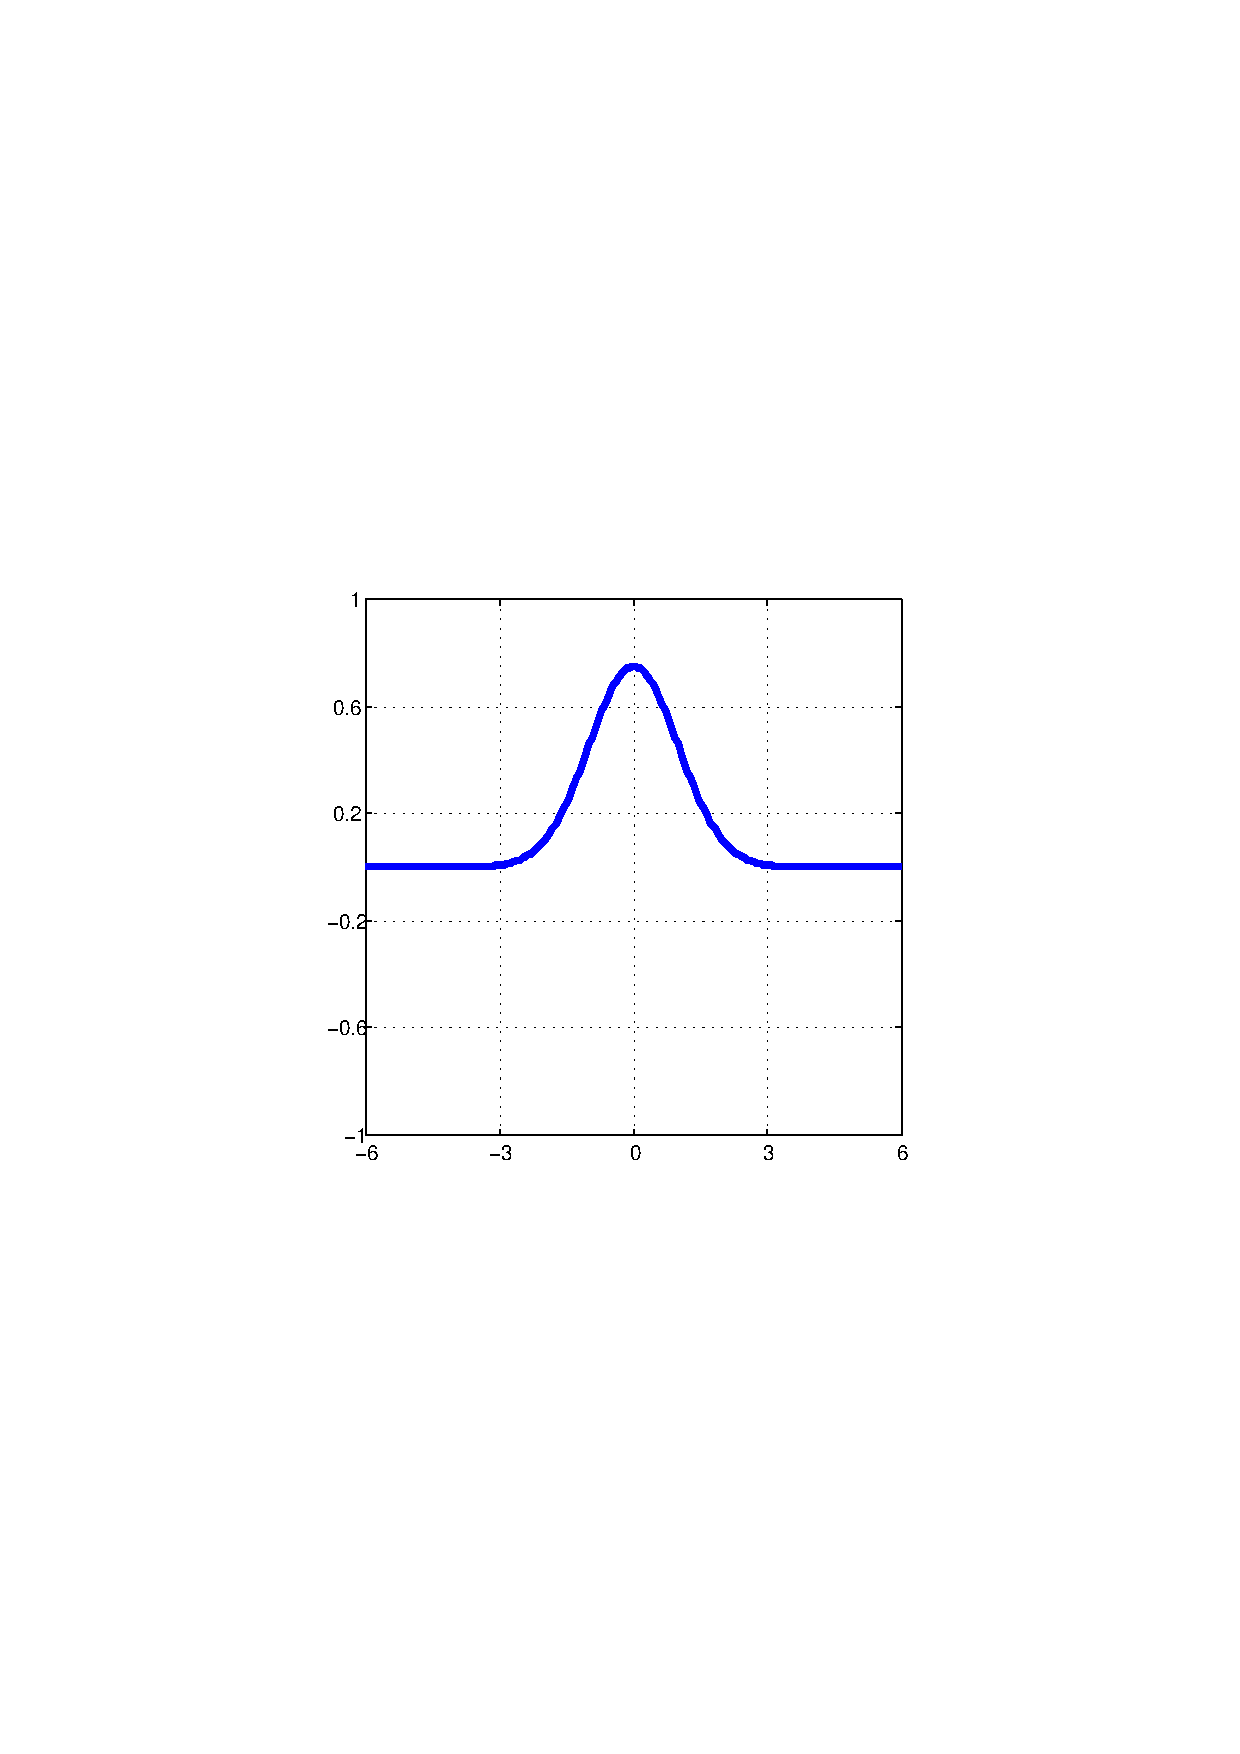
\includegraphics[scale=0.34,trim=150 280 150 280,clip]{./%Abrak/Egyeb/phi0.pdf}} 
%\subfigure[$\Phi_{1}(x)$]{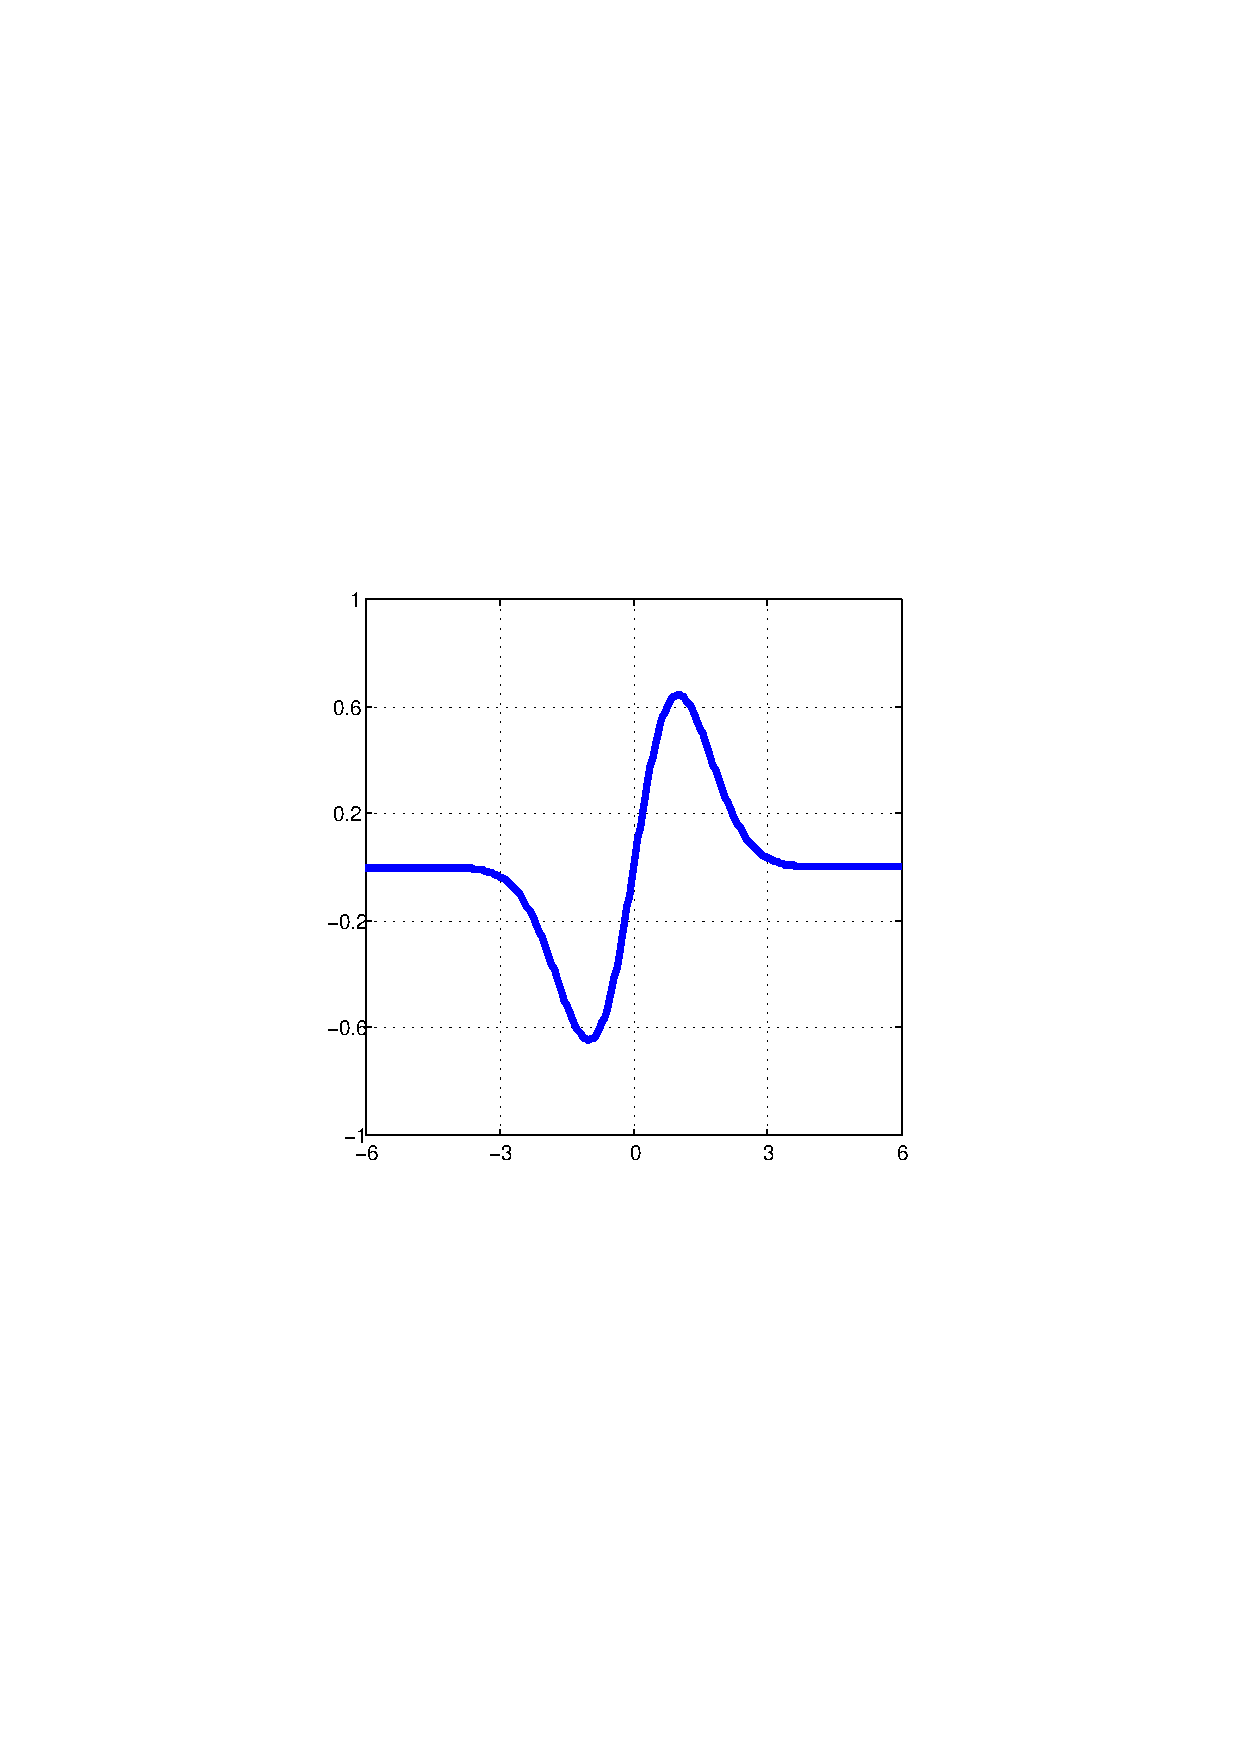
\includegraphics[scale=0.34,trim=150 280 150 280,clip]{./%Abrak/Egyeb/phi1.pdf}}
%\subfigure[$\Phi_{2}(x)$]{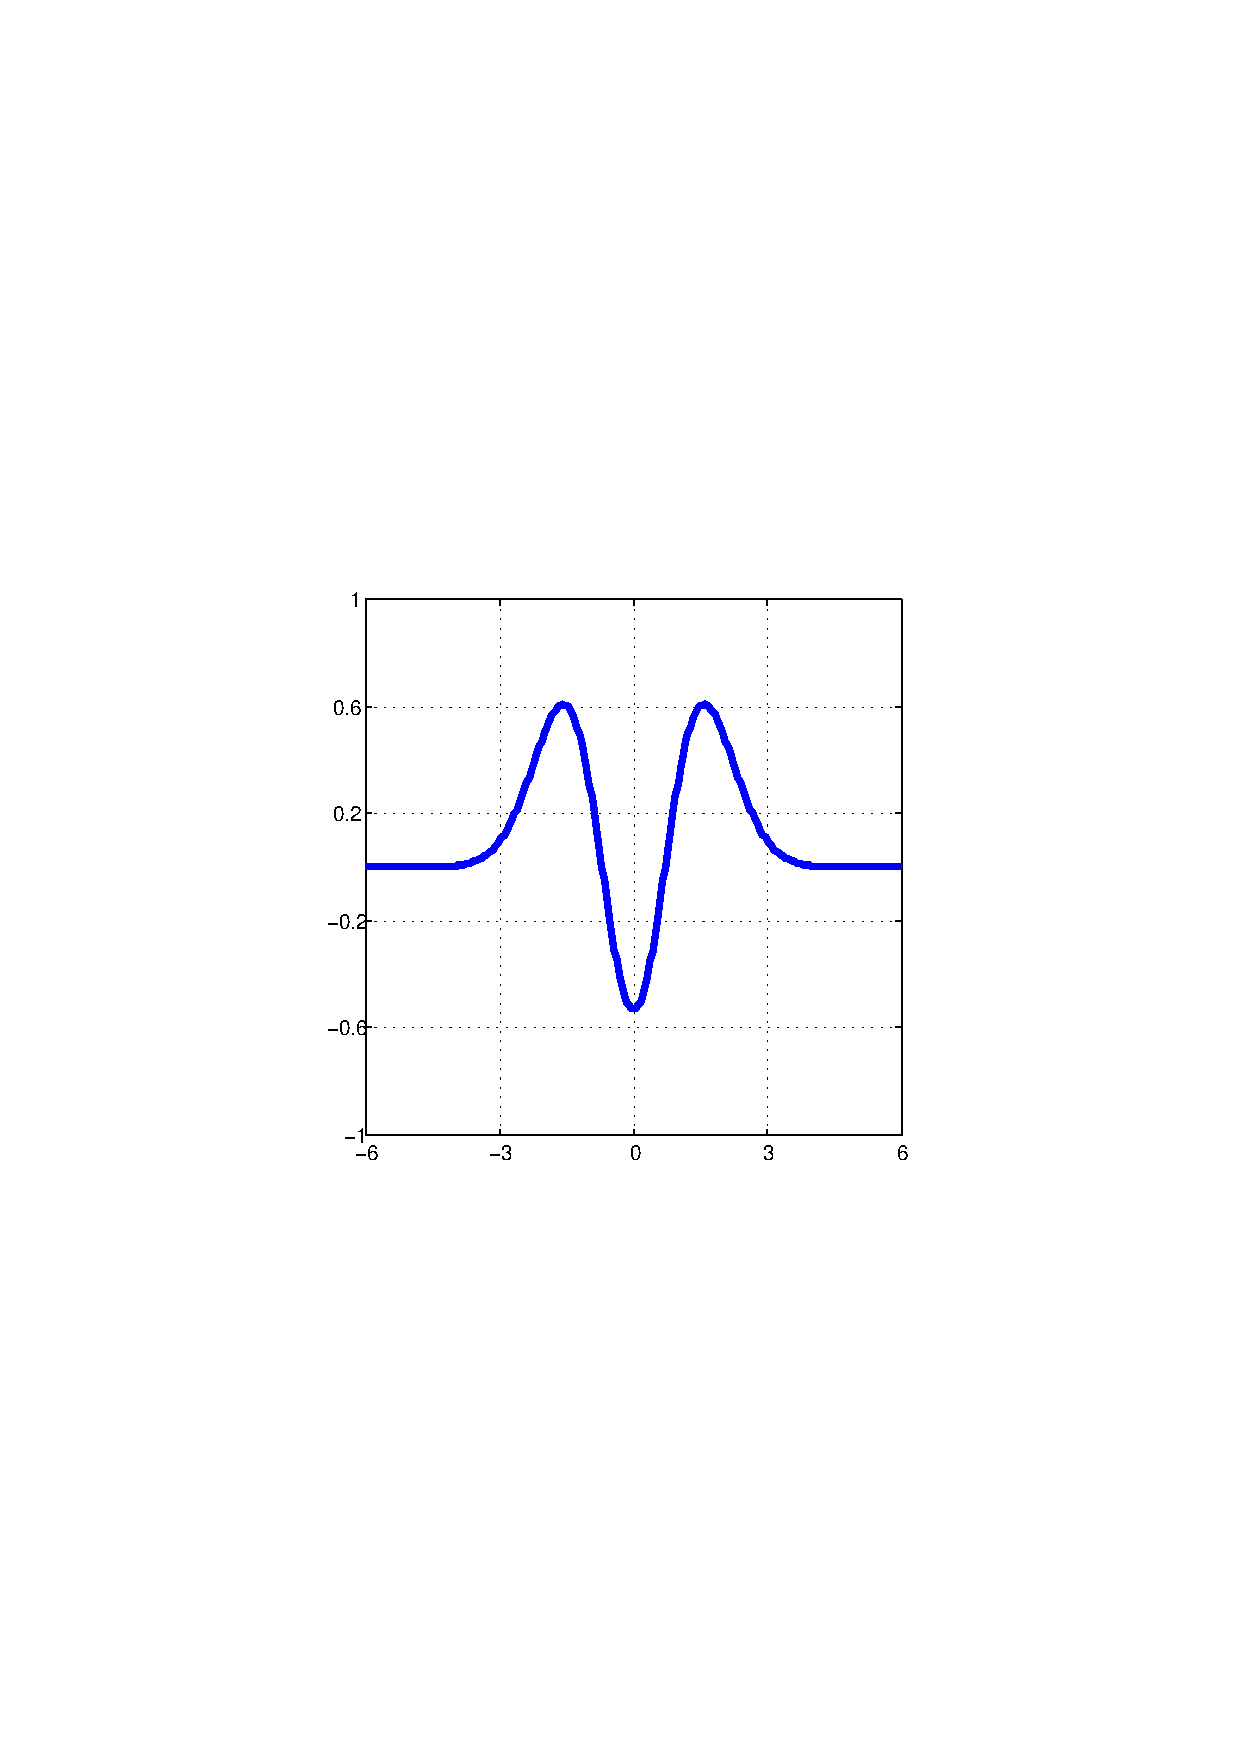
\includegraphics[scale=0.34,trim=150 280 150 280,clip]{./%Abrak/Egyeb/phi2.pdf}} 
%\subfigure[$\Phi_{3}(x)$]{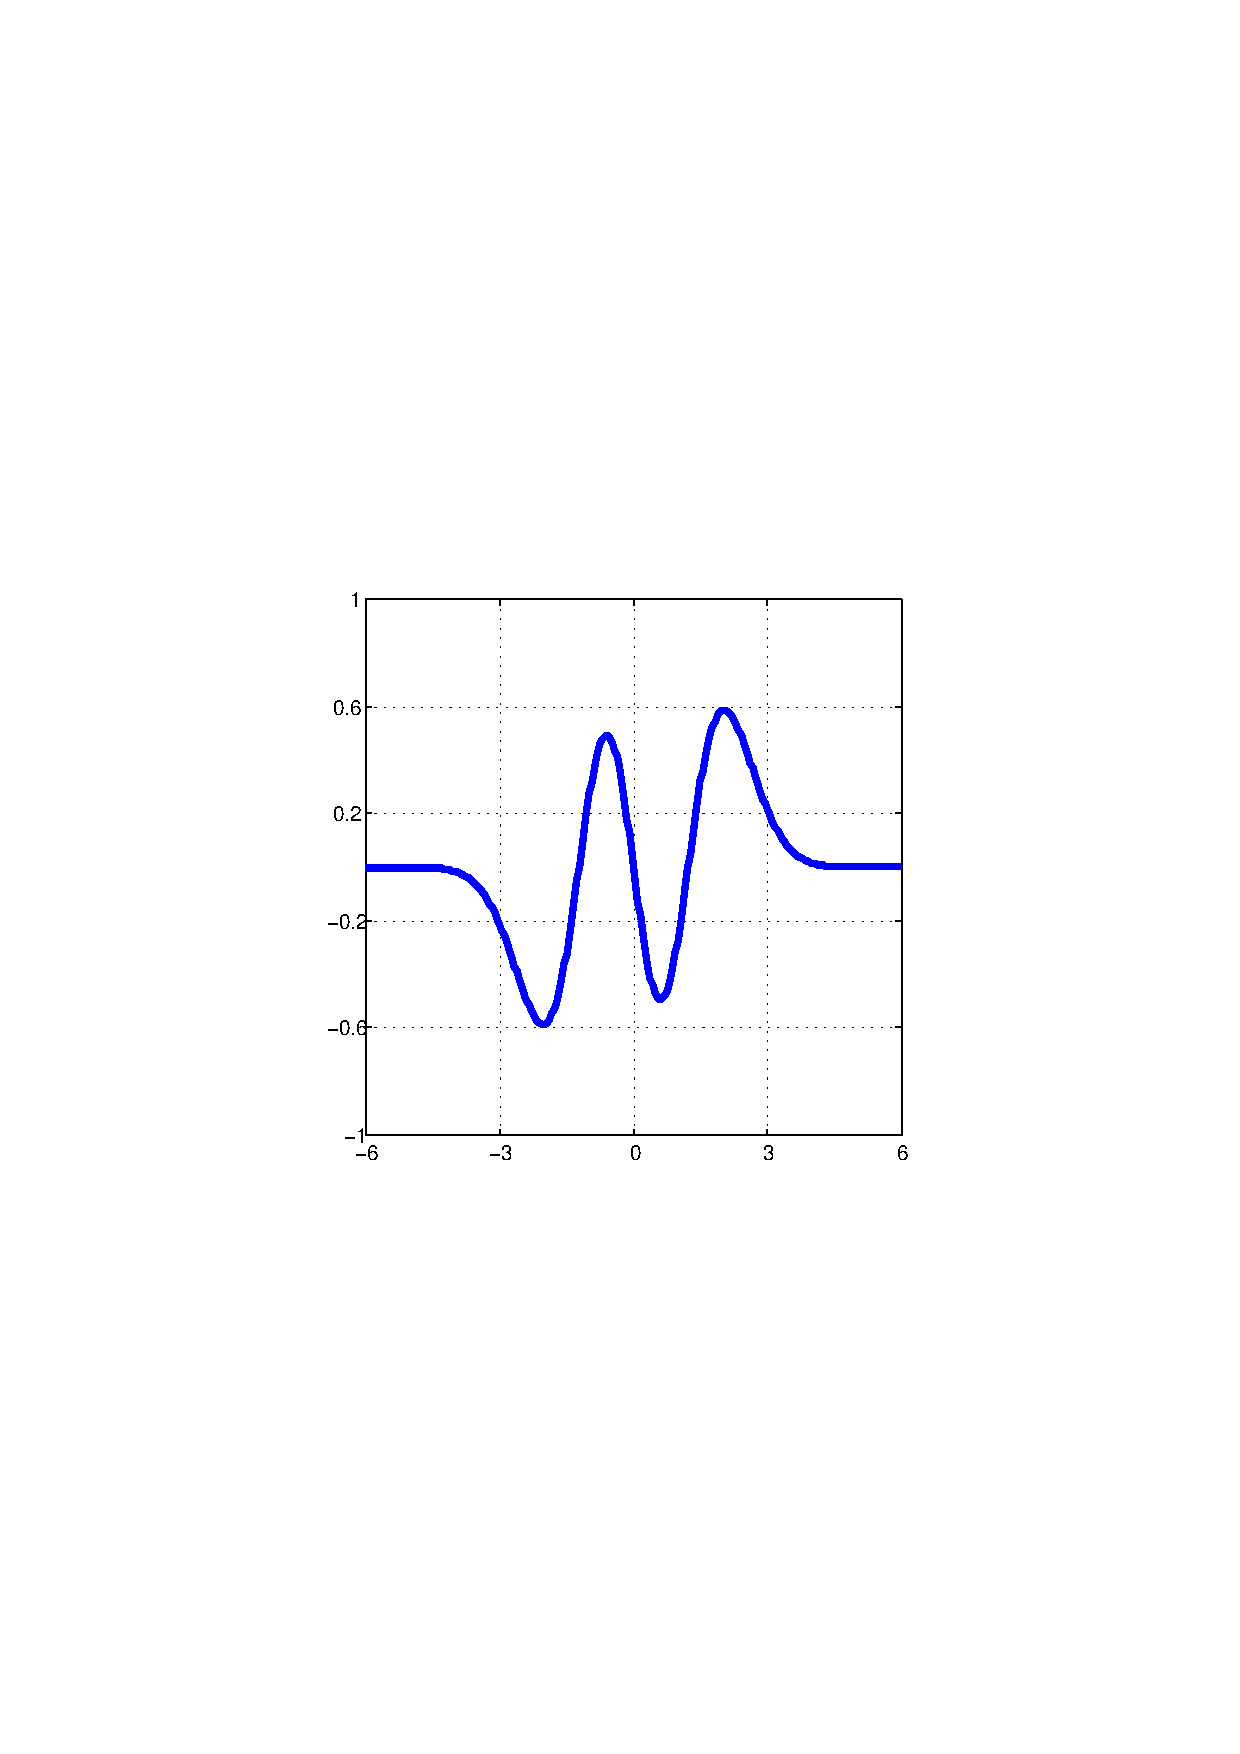
\includegraphics[scale=0.34,trim=150 280 150 280,clip]{./%Abrak/Egyeb/phi3.pdf}}
%\caption{A Hermite-függvényrendszer első négy tagja.}
%\label{fig:phi0-3}
%\end{figure}

\subsection{Hermite-függvények}
A dolgozatban  az $\Bbb R$ számegyenesen (Lebesgue-mérték szerint) négyzetesen integrálható függvények $\mathcal H$ Hilbert-tere helyett elegendő a szakaszonként folytonos, az $\Bbb R$-en  négyzetesen integrálható függvények $\mathcal F$ euklideszi terét használni. Ebben a térben a skaláris szorzat és a norma a következő alakban írható fel:
\begin{equation}
 \langle f,g\rangle:=\int_{-\infty}^\infty f(t)g(t)\, dt,\ \ \|f\|:=\sqrt{\langle f,f\rangle}\ \ (f,g\in\mathcal F)\,.
\label{eq:dotprod}
\end{equation}
Továbbá, a
 \begin{equation*}
 \Phi_n(x):=H_n(x)e^{-x^2/2}/\sqrt{\pi^{1/2}2^n n!}\quad \ (n\in\Bbb N)
 \end{equation*}
normált Hermite-függvények (teljes) ortonormált rendszert alkotnak az $\mathcal F$ téren:
  \begin{equation*}
   \langle \Phi_n,\Phi_m\rangle=\delta_{nm}\ \ (m,n\in\Bbb N),\quad
  \|f-S_nf\|\to 0\ (n\to\infty)\,.
   \end{equation*}
Itt $H_n\ (n\in\Bbb N)$ jelöli az Hermite-féle polinomokat.
\\
\\
Az Hermite-függvények alkalmazásának számos előnye van: \\
\\
i) A $\Phi_n\ (n\in\Bbb N)$ rendszer zárt (teljes) az $\mathcal F$ téren. \\
\\
ii) A $\Phi_n(x)$ függvények gyorsan tartanak $0$-hoz, ha $|x|\to \infty$: \\
$$
|\Phi_n(x)|\le M_n e^{-x^2/4}\le M_n\ \ (x\in\Bbb R, n\in\Bbb N).
$$
\\
iii) A $\Phi_n$ függvények (stabil) másodrendű rekurzióval számíthatók: \\
\begin{equation}
\begin{split}
&\Phi_0(x):=e^{-x^2/2}/\pi^{1/4},\ \Phi_1(x):=\sqrt{2}\, x e^{-x^2/2}/\pi^{1/4}\\
&\Phi_n(x)=\sqrt{\frac 2 n} x \Phi_{n-1}(x)-\sqrt{\frac{n-1}n}\Phi_{n-2}(x)\ \ (x\in\Bbb R, n\ge 2)
\end{split}
\end{equation} 
\\
\\
iv) A $\Phi_n'$ deriváltak kifejezhetők a $\Phi_n, \Phi_{n-1} $ függvényekkel: \\
\begin{equation}
\Phi_n'(x)=\sqrt{2n}\Phi_{n-1}(x)-x\Phi_n(x)\ \ (x\in\Bbb R, n\in\Bbb N,\Phi_{-1}=0)
\end{equation}

\section{Az approximáció optimalizálása}

A jelek reprezentációja  függ az időskála $0$ pontjának és az egység
megválasztásától. Ezeket a paramétereket  a gyakorlatban önkényesen szoktuk
 megválasztani. Ezzel összefüggében felvethető a kérdés, hogyan lehet optimálisan megválaszthatani  ezeket a paramétereket.
Az  approximáció pontosságát javí thatjuk azonos együttható szám mellett, amennyiben az  Hermite-függvények helyett azok
\begin{equation}
\Phi_n^{a,\lambda}(x):=\Phi_n(\lambda x+a)\ \  (x,a\in\Bbb R, \lambda>0)
\end{equation}
affin transzformáltjait használjuk. A $\sqrt{\lambda}\Phi_n^{a,\lambda}\ (n\in\Bbb N)$ rendszer is ortonormált és teljes az $\mathcal F$ téren. Ebben az esetben
az $f$ legjobb approximációja az
\begin{equation}
S_n^{a,\lambda}f:=\sum_{k=0}^n\langle f,\Phi_k^{a,\lambda}\rangle\Phi_k^{a,\lambda}\ \
(n\in\Bbb N, a\in\Bbb R,\lambda>0)
\end{equation}
projekció és a közelí tés hibája az $a$ transzlációs és a $\lambda$ dilatációs paraméter függvénye:
\begin{equation}
D^2_n(a,\lambda):=\|f\|^2-\sum_{k=0}^n|\langle f,\Phi_k^{a,\lambda}\rangle|^2.
\end{equation}
            E két szabad paraméter optimalizálásával azonos együtthatószám mellett, az eredeti Hermite polinomokkal törtánő  approximációhoz képest pontosabb közelí tést érhetünk el. A $D_n$ függvény minimalizálása ekvivalens  az
 $$
 F_n(a,\lambda):=\sum_{k=0}^n|\langle f,\Phi_k^{a,\lambda}\rangle|^2
 $$
 függvény maximumának meghatározásával. A paraméteres integrálok tulajdonságaiból következik, hogy az
 $$
 A_n(a,\lambda):=\langle f,\Phi_k^{a,\lambda}\rangle \ \  ((a,\lambda)\in T:=\Bbb R\times (0,\infty))
 $$
 Fourier-együtthatók a $T$ tartományon a paraméterek sima függvényei. Bebizonyí tható, hogy $\lambda\to 0$ és $|a|+\lambda\to \infty$ esetén
 $F_k(a,\lambda)\to 0$, következésképpen az $F_n$ függvénynek létezik a
 maximuma és a $D_n$ függvénynek létezik a minimuma. A részleteket a Függelékben találhatók.

 Az alábbi ábrák az $F_n(a,\lambda)$ függvényeket szemléltetik fényintenzitás és perspektivikus ábrázolást használva. A harmadik ablakon
a jel közelí tését szemlélteti a maximum helynek megfelelő, ill.  egyéb
paraméter esetén.

\begin{figure}[H]
\begin{center}
   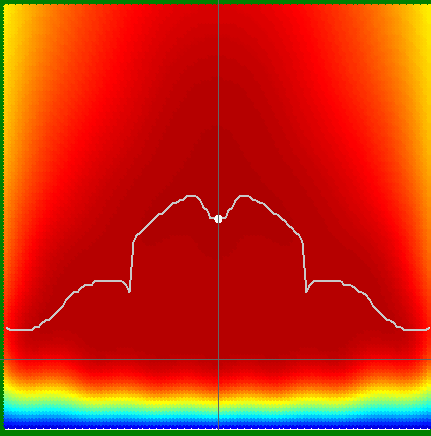
\includegraphics[width=100mm]{./Abrak/Ereszkedo1/F_2sz.png}
  \caption{Az $F_n$ szí nkódos ábrázolása}
\end{center}
\end{figure}

\begin{figure}[H]
\begin{center}
   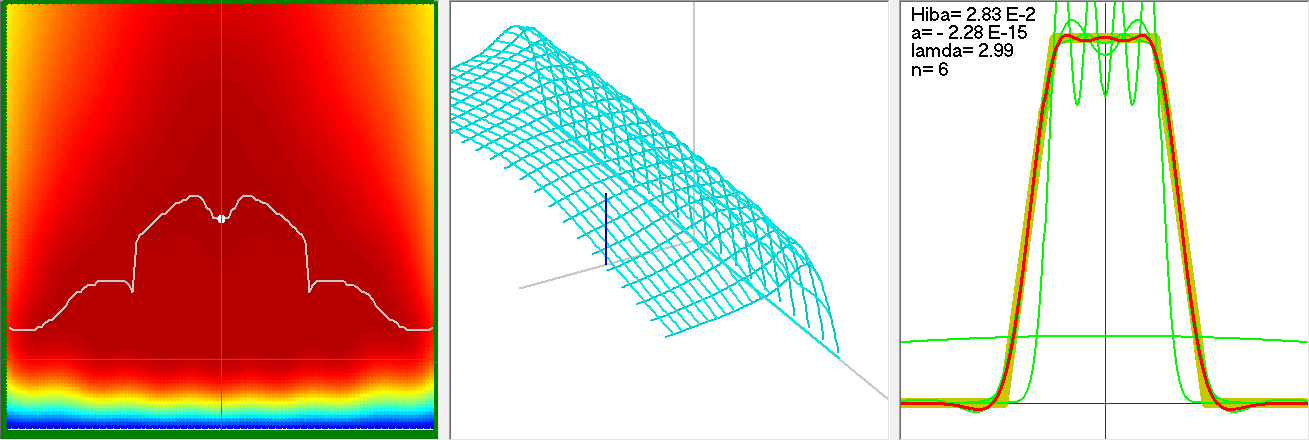
\includegraphics[width=140mm]{./Abrak/Ereszkedo1/Er36.png}
  \caption{Az $F_n$ által meghatározott felület, és approximáció}
\end{center}
\end{figure}


\chapter{Felhasználói dokumentáció}

\chapter{Fejlesztői dokumentáció}

\end{document}
